% Drawing 69/06-11 -- folder 69, batch 06, archive page 119 (PDF page 120).
% Transcription: en haut, une courbe fermée allongée avec une double flèche ; un « $V$ » dans un parallélogramme ; une ellipse traversée d'une courbe, hachurée sur un bord
% Kind: closed curve with double arrow; V in a parallelogram; ellipse crossed by a curve. Method 2 (schematic redraw from the facsimile). Status: partial.
% Notes: Upside-down half of the sheet (crop rotated 180 degrees, redrawn upright). At the top: an elongated closed curve with a short double arrow at its right end; a V, its left stroke ending in an arrowhead, beside a parallelogram drawn open (a long lower side, a short stroke rising at its left end, the right side and a short upper stroke at the right, as on the page); a tilted ellipse crossed by two heavy strokes (one from its upper left end down to the right, one curving down from the upper right to the lower left), with short hatching strokes on its upper right edge. Not drawn: the text (Gamma -> S^1, S^2 x S^2 - diag ...) and the long diagonal strokes across the sheet. Redrawn 2026-11-09 (issue 128). Overlay check 2026-11-13 (claude-opus-5-5, issue 147): the 300 dpi colour rendering of the 250 ppi scan laid under the redraw, rasterised from its TikZ (not compiled: no TeX in the session). The closed curve was 2 units low and short at its right end, the V and the parallelogram 1 to 2 units off and of another shape (the V had no arrowhead, the parallelogram a closing stroke the page does not have), the ellipse 2 units too far to the lower left: all redrawn through points read on the scan; the single heavy stroke across the ellipse is two strokes on the page, both drawn; the hatching strokes moved by up to 1 unit. Still differs: the ellipse is a freehand loop whose upper left part is overinked and merges with the first heavy stroke, so its outline there is a reading (within about 1 to 1.5 units); the lower head of the double arrow is a small V on the page.
% Coordinates: 1 unit = 1 mm = 1/100 of the crop width (bbox in page fractions: [0.08, 0.15, 0.95, 0.86]).
% Redrawn by Claude (claude-opus-5-5), issue #73, 2026-11-09; not checked by a human; not compiled (no TeX in the session).
% Checked by Claude (claude-opus-5-5) 2026-11-13 (issue #147): overlaid on the colour scan (250 ppi, rendered at 300 dpi) and corrected; not compiled (no TeX in the session), rasterised for the overlay by a Python reader of this TikZ. Status: partial.
% Rights: reproduces part of the work -- behind RENDER_TRANSCRIPTS, never published by itself.
\documentclass[tikz,border=3pt]{standalone}
\usepackage{amsmath,amssymb}
\usetikzlibrary{patterns,arrows.meta}
\tikzset{pencil/.style={black!45}, struck/.style={black!35}, mark/.style={circle,draw,inner sep=1.3pt}, pt/.style={circle,fill,inner sep=0.9pt}, opt/.style={circle,draw,fill=white,inner sep=1.1pt}}
\begin{document}
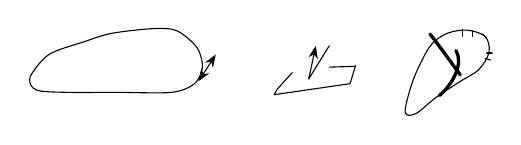
\begin{tikzpicture}[x=1mm,y=1mm,line cap=round,line join=round,font=\scriptsize]
\draw plot[smooth cycle, tension=0.5] coordinates {(23,-8.2) (25.4,-5.3) (29.8,-3.7) (33.4,-2.6) (38.8,-2) (41.7,-2.3) (44.2,-4.4) (44.9,-6.9) (43.9,-9) (41,-10.1) (34,-10.1) (27.6,-10.1) (23.8,-9.8)};
\draw[{Stealth[length=1.6mm]}-{Stealth[length=1.6mm]}] (44.4,-8.7) -- (46.6,-5.3);
\draw[-{Stealth[length=1.6mm]}] (58.4,-8.4) -- (59.3,-4.2);
\draw (58.4,-8.4) -- (61,-4.2);
\draw (56.3,-7.6) -- (54.4,-9.7) -- (54,-10.4) -- (63.65,-9) -- (64.35,-6.7);
\draw (61,-6.9) -- (64.2,-6.8);
\draw plot[smooth cycle, tension=0.55] coordinates {(70.65,-12.6) (71.5,-9) (72.8,-6) (74.1,-3.9) (76,-2.6) (78.5,-2.2) (80.8,-3) (81.3,-5) (80,-7.2) (77.5,-8.8) (74.5,-10.8) (72,-12.8)};
\draw[very thick] (73.8,-2.7) .. controls (75,-4.2) and (76.4,-6.2) .. (77.65,-7.9);
\draw[very thick] (77.1,-4.8) .. controls (78,-6.2) and (77,-8.8) .. (75,-10.5);
\draw (77.9,-2.1) -- (77.9,-3);
\draw (79.2,-2.3) -- (79.2,-3);
\draw (80.5,-2.7) -- (81,-3.2);
\draw (81,-5.1) -- (81.7,-5.1);
\draw (80.8,-5.8) -- (81.5,-6);
\end{tikzpicture}
\end{document}
